\section{The Ghost-Separation Formula}

\subsection{Building the Intuition First}

Picture two pinholes, side by side, separated by a distance $s$ (their
center-to-center pitch). Light from a single point far away enters both
holes. If the eye's lens is perfectly focused for that light, both holes'
worth of light converges to \emph{exactly the same spot} on the retina ---
this is just what ``in focus'' means: parallel rays entering a lens at
different positions still meet at one point.

Now suppose the eye is short-sighted by $M$ diopters --- the lens converges
light slightly too much (or too little) for that point to land exactly on
the retina. The image plane is now displaced from the retina by a small
amount related to $M$. Each hole, because it sits at a different lateral
position, now projects its slightly-out-of-focus point to a \emph{slightly
different} spot on the retina. The two images are no longer perfectly
overlapping.

\intuitbox{The key physical fact that makes this predictable: the size of that
retinal offset grows in direct proportion to \emph{both} the hole
separation $s$ \emph{and} how far out of focus the eye is ($M$). Zero
separation, or zero defocus, means zero offset --- there is nothing subtle
here, it is basic similar-triangles geometry once you draw the ray paths
through the eye's lens.
}
\subsection{The Formula}

The validated closed-form result used throughout this project is:
\begin{equation}
\Delta r = \frac{s \cdot M}{P_0 - M}
\end{equation}
where $s$ is the hole-to-hole separation, $M$ is myopia in diopters, and
$P_0$ is the eye's total optical power (a fixed constant of the eye model,
$\approx 60$D). Notice the formula automatically gives $\Delta r = 0$ when
$M=0$ --- exactly the ``in focus, both holes agree'' case described above.
This is not a coincidence; it is the formula correctly reproducing a case we
already know the answer to by pure geometry, which is one of the strongest
kinds of sanity check available in physics.

An earlier, uncorrected version of this formula was used in this project
before it was properly checked. It did \emph{not} go to zero at $M=0$,
which on its own was enough to know it was wrong --- a formula that
disagrees with a case you can reason out by hand needs no further testing
to be rejected.

\subsection{How the Correct Formula Was Actually Confirmed}

Rather than trust either candidate formula on paper, this project built an
independent test: place exactly two holes in a real wave-optics simulation
(not a formula --- an actual propagation of light through the eye model),
measure where the two resulting bright spots land on the simulated retina,
and see which formula's prediction matches. Figure~\ref{fig:ghostvalid}
shows the result: the corrected formula fits the directly-measured data
with $R^2 = 0.995$ (essentially perfect agreement), while the old formula
scores $R^2 = -1701.7$ --- a negative $R^2$ means the old formula was
\emph{worse than simply guessing the average value every time}, which is
about as decisively wrong as a formula can be shown to be.

\begin{figure}[h]
\centering
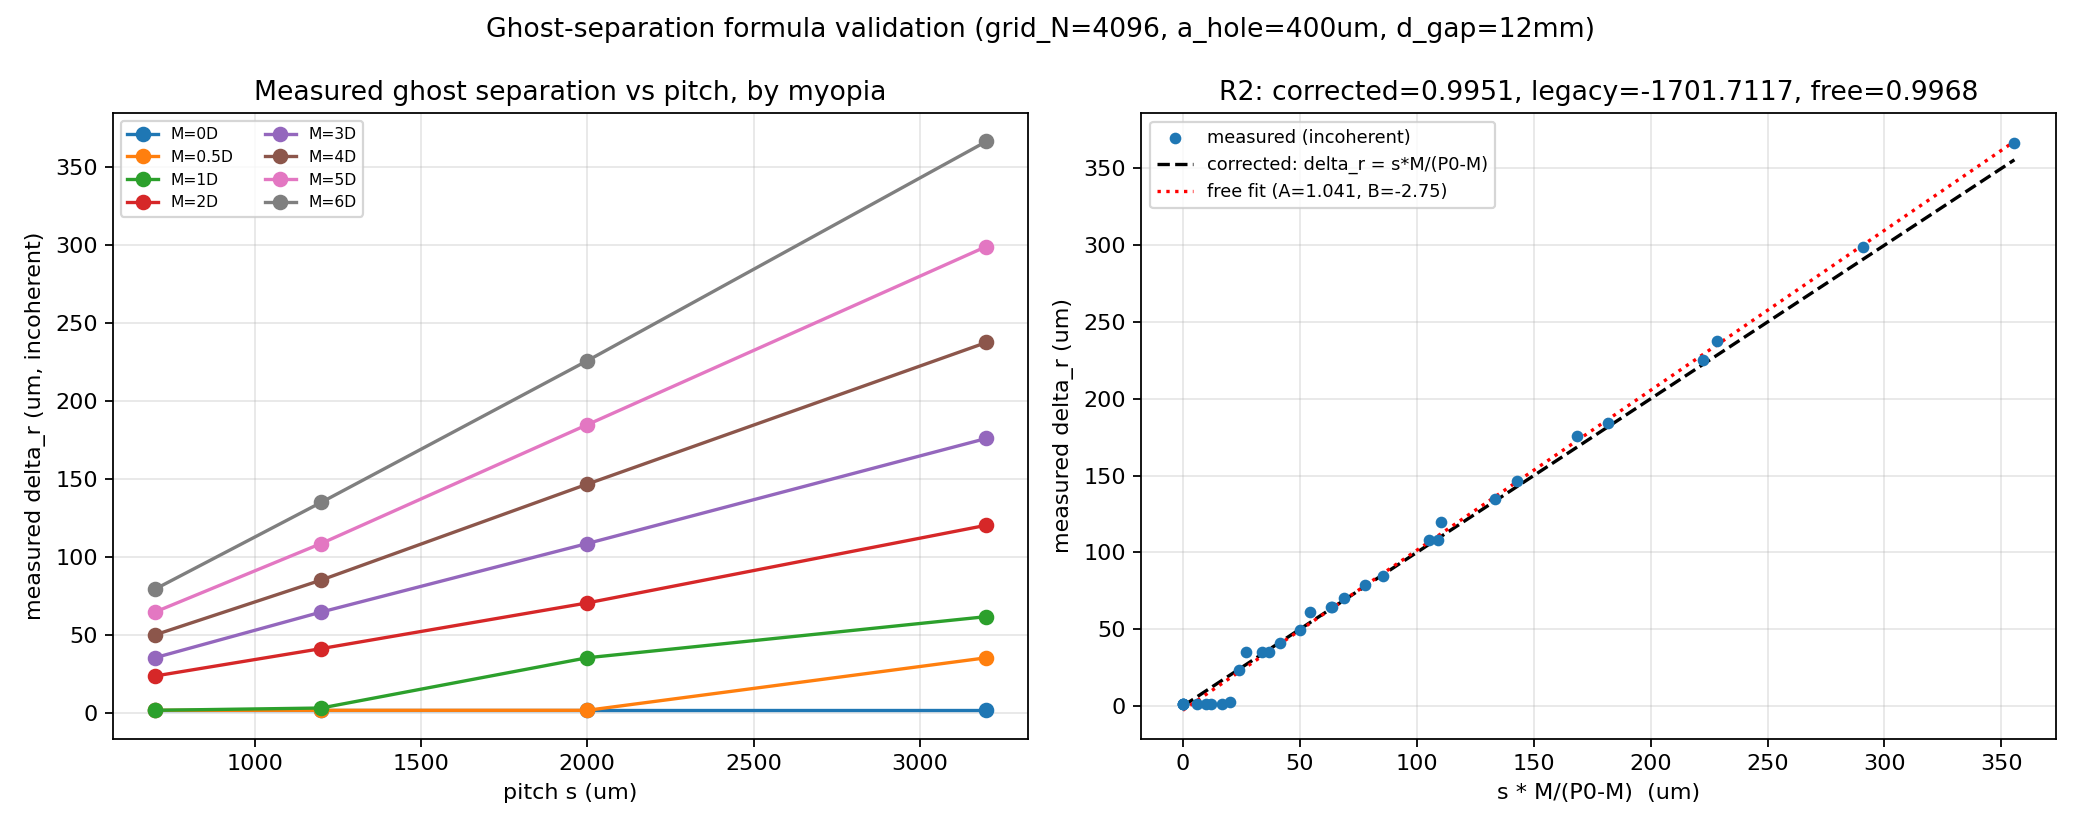
\includegraphics[width=0.85\textwidth]{handbook_figs/ghost_formula_validation.png}
\caption{Directly-measured ghost separation (from real two-hole wave-optics
propagation) versus both candidate formulas. The corrected formula
($R^2{=}0.995$) is the one used throughout this project's array code; the
legacy formula ($R^2{=}-1701.7$) is not.}
\label{fig:ghostvalid}
\end{figure}

\codemapbox{The formula itself lives in \texttt{array\_geometry\_lab/degeneracy\_filter.py}
and \texttt{array\_optimization/stage0\_ghost\_validation/} (the original
validation, copied for speed into the geometry-comparison pipeline so it can
be evaluated thousands of times without re-running full wave optics each
time). The safety rule built on top of it is simple: for every pair of
holes that could be simultaneously lit by the pupil, compute $\Delta r$; if
the eye's own ability to resolve two separate points is smaller than every
$\Delta r$ in the pattern, the design is ghost-safe. This is
\texttt{gate\_ghost\_safety()} in \texttt{comparison\_metric/gates.py}.
}
\newpage
